\section{これまでの成果}
\label{sec:progress}

本研究は現時点では新規の回路提案や測定を行う段階には至っておらず，第\ref{sec:proposal}節で述べた比較検討を行うための土台を整備する段階にある．これまでに行った作業は，大きく以下の2点である．

\subsection{既存最適化プログラムの再現}

まず，先輩から提供を受けたMATLABプログラム（NSGA-IIに基づく多目的最適化フレームワーク\cite{zhu_moea_2025}の実装）を実行し，論文中と同様のジッタ・電力パレートフロントが得られることを確認した．図\ref{fig:pareto-compare}に，DTCベースPLLとHMベースDual-Feedback PLLのジッタ・電力トレードオフを比較したパレートフロントを，図\ref{fig:pareto-final}に最適化計算の最終結果の一例を示す．いずれも先輩のプログラムをそのまま実行して得たものであり，フレームワークの動作を自身の手元で確認できたことを意味する。

\begin{figure}[H]
  \centering
  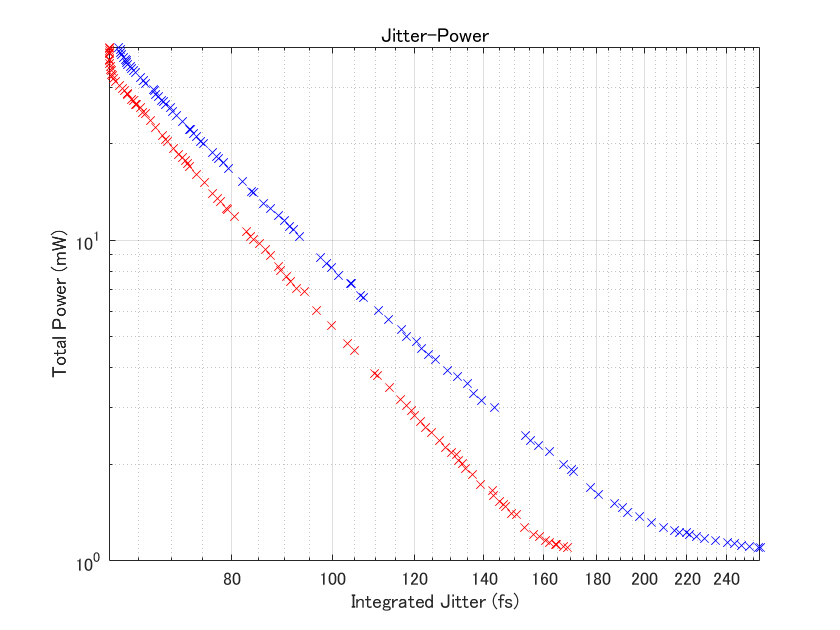
\includegraphics[keepaspectratio,width=0.8\columnwidth]{fig/matlab_pareto_compare.png}
  \caption{既存プログラムによるジッタ・電力パレートフロントの再現例（2アーキテクチャの比較）．}
  \label{fig:pareto-compare}
\end{figure}

\begin{figure}[H]
  \centering
  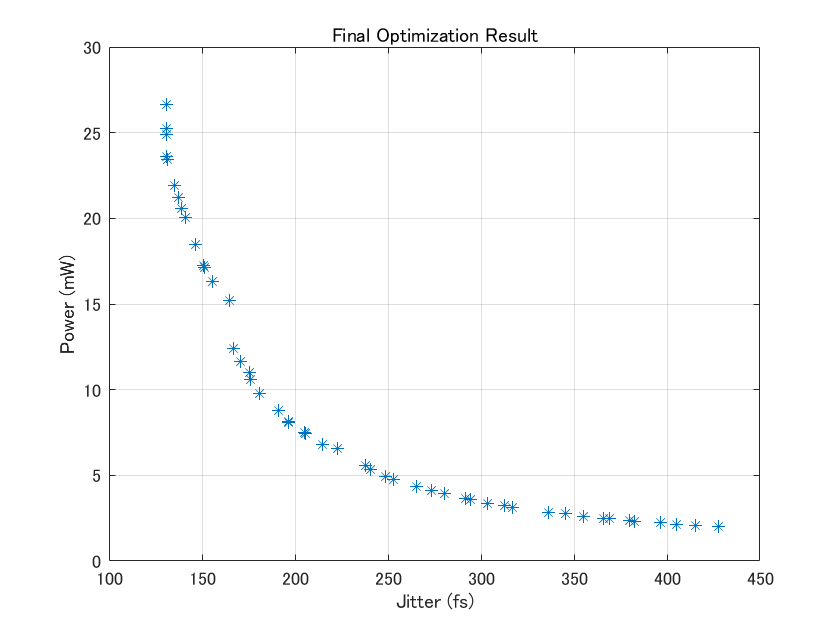
\includegraphics[keepaspectratio,width=0.8\columnwidth]{fig/matlab_pareto_final.png}
  \caption{NSGA-IIによる最適化計算の最終世代の結果例（ジッタ vs 消費電力）．}
  \label{fig:pareto-final}
\end{figure}

\subsection{フィードフォワード型構成の理解とモデル化に向けた準備}

次に，第\ref{sec:methods}節で紹介したフィードフォワード型構成\cite{zhang_ffnc_2025}の技術内容の理解を進めた．位相検出器のゲインやループフィルタの伝達関数（原論文の式(6)・式(7)に相当する部分）については，導出過程を自分の手で追い直し，内容を確認できた．一方で，補助PLLから出力までの伝達関数（原論文の式(8)以降，フィードフォワードによるキャンセル項を含む部分）については，式の導出過程に理解が及んでいない箇所が残っており，この部分をノイズ解析モデルへ正確に反映するところまでは至っていない。

並行して，Dual-Feedback構成において，補助（外部）PLLの雑音寄与を主ループの雑音源（基準・PD・ループフィルタ・VCO・DSM量子化雑音）から分離し，それぞれの積分ジッタへの寄与率を算出できるMATLABモデル（\texttt{DualFF\_typeI\_typeII\_lag\_lead\_lag.m}）を構築した。ただし，このモデルは現時点ではフィードフォワードによるキャンセル項を含んでおらず，キャンセルを行わない状態での補助PLL寄与を可視化するにとどまっている。

% TODO: DualFF_typeI_typeII_lag_lead_lag.m を実行して得られる位相雑音特性カーブ（figure 1, figure 2：補助ループ・主ループそれぞれのノイズ寄与内訳）をここに貼る。
% \begin{figure}[H]
%   \centering
%   \includegraphics[keepaspectratio,width=0.8\columnwidth]{fig/dualff_phase_noise.png}
%   \caption{補助PLLの雑音寄与を分離したノイズ解析モデルの出力例．}
%   \label{fig:dualff-pn}
% \end{figure}

フィードフォワード型構成のジッタ・電力への効果を定量的に評価するには，このキャンセル項をモデルに導入する必要があり，これが直近の課題である（第\ref{sec:future}節）。
